\chapter{Computing}
One important notion of compute system is \textit{density}: there are different needs (in how many cores / how many operations per second) depending on the application that is running on the system. The structure of a server is a tradeoff between \textbf{capacity} (even if we need to do a lot of computing, space is limited, so less space for the drives) and \textbf{density}.

{
   There are two types of compute systems in a datacenter:\ns
   \begin{enumerate}
   \item \textbf{Rack} servers: they are the most common type of servers, and are used for general purpose applications.
   \item \textbf{Blade} servers: they are used for specific applications, and are more expensive than rack servers.
   Each blade server is a self-contained compute system, inserted in a ---fatter--- \textit{chassis}, typically dedicated to a single application, providing multiple services.\\
   The modular design of blade server make them smaller, minimizing floor space requirements, increasing system density and scalability, ultimately providing a more efficient use of power and cooling, compared to tower and rack servers.
   \note{Usually contain only CPU(/RAM) and NIC, but in some cases also storage, possibly configured as SAN or NAS.}
   \end{enumerate}
}

\section{Remote Management of servers}
\begin{center}
   ``In a server how many OSs are ran at the same time?''
\end{center}
2 in general, one is \ul{``Base Management Console''}\footnote{May have other names, but this is a common one, used by \texttt{Supermicro}}.

The BMC is a full OS running in a board which executes also when the server is off, but attached to a power supply. It is a component which allows you to manage the server as if you were phyisically handling the server.

Prof. Cisternino display iDRAC (Dell's BMC) in class. It is a web interface which allows you to manage the server, check its status, and even turn it on and off. \\
It is also possible to access a console, which is a virtual console, which allows you to interact with the server as if you were physically there with keyboard and mouse attached;
such console also allows to install a new OS by uploading an \texttt{iso} and make the server boot from it as if it was attached to it.
\begin{figure}[htbp]
   \centering
   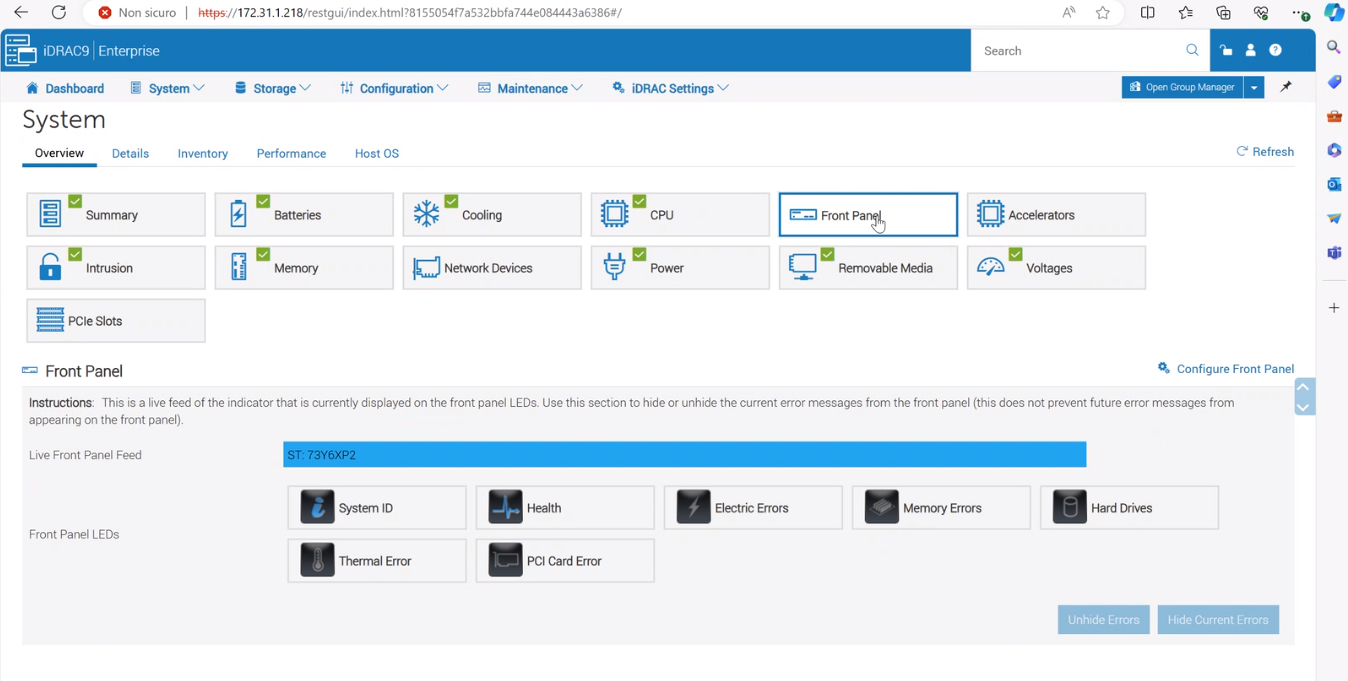
\includegraphics{images/monitoring_servers.png}
   \caption{DEMO Interface displayed by prof cisternino in class}
   \label{fig:monitoring_servers}
   It is possible to remotely control and check the server's status.
\end{figure}

\begin{figure}[htbp]
   \centering
   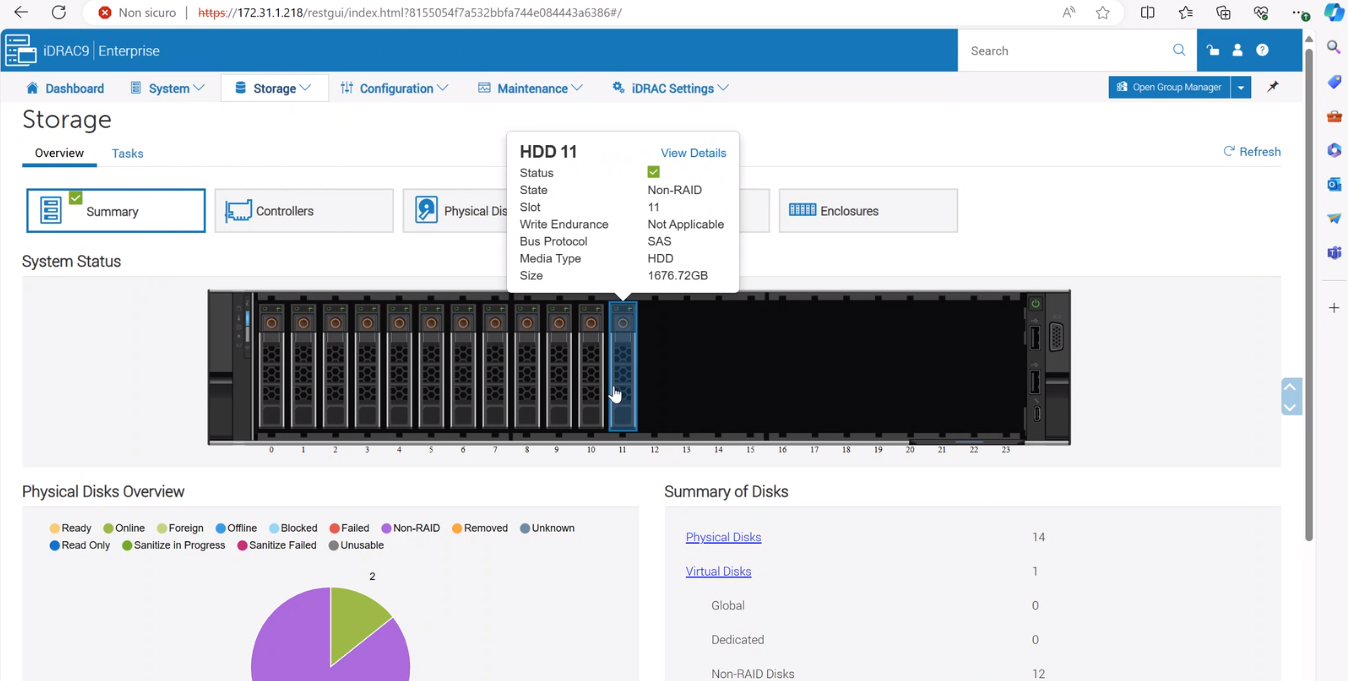
\includegraphics{images/monitoring_servers2.png}
   \caption{Monitoring storage}
   \label{fig:monitoring_servers2}
   SAS bus protocol is used for storage devices.
\end{figure}

\note{CPU Affinity of a RAM bank indicates which CPU is connected to that bank.}

The BMC typically has a dedicated network interface, which is used to connect to the server, separated from the standard network interface.
Redfish is a standard which is used to manage servers. It is a RESTful API which allows to manage servers and automate some tasks.

\framedt{Predict Storage failure}{
   A disk may fail without any prior notice, at any time, just like a heart attack.
   However there are some signs which may indicate that a disk is about to fail;
   these are detected by the \textit{Smart} technology.
   Also AI may be used to predict disk failure.
}
\nl

\begin{center}
   \textit{No phyisical security means no security at all}
\end{center}
The BMC is very useful because allows for administrators to manage server remotely, without having to physically access the server.
This is not only ``handy'', but often necessary, since the \ul{\textit{physical} security of the datacenter must be high}, and not everyone should be allowed to access the server room.

\framedt{Measuring Bus Speed}{
   PCIe speed, as well as CPU speed is measured in GT/s, which stands for \textit{Giga Transfers per second}. It is a measure of how many transfers can be performed in a second.
}

\section{Knights Landing and high performance computing}
\textbf{Knights Landing} is an old multi ---up to 72--- core architecture designed to be used in supercomputers. The memory had a super high bandwidth, to avoid bottlenecking the many cores inside, since such memory is shared among them.

\textit{NUMA} is a technique used to avoid bottlenecking in multi core architectures. It is a technique which allows to have multiple memory banks, each one connected to a subset of the cores. This way, each core can access its own memory bank without having to wait for the others to finish accessing the shared memory.



\section{Rings}
Bachelor's professors fooled us into thinking that CPUs have two operating modes, \textit{user} and \textit{kernel} mode. Sadly, this ain't true, it is an abstraction. In reality,\ul{ CPUs have 4 \textbf{rings}}, which are used to separate the different levels of privilege. The higher the ring, the higher the privilege level.
The kernel runs in ring 0, while the user runs in ring 3.

Nowdays there are multiple units in the CPU, which are used to execute instructions, and there is a head unit which decides which instruction to execute next and on which unit.

Chiplets are a way to increase the number of cores in a CPU. They are small chips which are connected to the main CPU.
Even at CPU the ``general-purpose'' methodology is not feasible anymore, and the CPU is divided into multiple units, each one specialized in a specific task.

\section{Misc notions on Hardware}
GPUs became of paramount importance for datacenter in the last years, mostly because of the rise of AI and machine learning. They are used to perform parallel computations, and are much faster than CPUs for such tasks.
However, they are very expensive.

NPUs (Neural Processing Units) are a new kind of processors, which hardware acceleration for for AI and machine learning tasks.
They are much cheaper than GPUs, and are becoming more and more popular.

\href{https://www.top500.org/}{TOP500} is a list of the 500 most powerful supercomputers in the world. It is updated twice a year, and is used to compare the performance of supercomputers.

